% reset section counter
\setcounter{section}{0}

%\metadata{lecture ID}{Your names}{date}
\metadata{10}{Kevin Han and Han Wu}{Feb 17th, 2021}

In the previous chapter, we outlined conceptual topics in deep learning theory and how the situation was different from classical machine learning theory. In particular, we described \textit{approximation theory}, \textit{statistical generalization} and \textit{optimization}. In this chapter, we will focus on optimization theory in deep learning. We will introduce some basics about optimization (Section~\ref{sec:optim_convergence}), discuss how we can make the notion ``all local minima are global minima'' rigorous, and walk through two examples where this is the case (Section~\ref{sec:two_optim_examples}). Finally, we introduce the neural tangent kernel approach which allows us to characterize of the loss of general neural networks near a specific initialization (or under specific parameterization).

\sec{Optimization landscape} \label{sec:optim_intro}

The big question that we have in mind is the following: many existing optimizers are designed for optimizing convex functions. \textbf{Why do they still work well empirically for non-convex functions?} We note that it is not true that these optimizers always work well with non-convex functions: there are still some very hard cases that give trouble (e.g. very deep feed-forward networks are still hard to fit because of issues like vanishing and exploding gradients). One possible reason is that the non-convex functions that we are minimizing in deep learning usually have some nice properties: see Figure \ref{lec10:fig:optimization} for an illustration.

\begin{figure}[ht!]
    \centering
    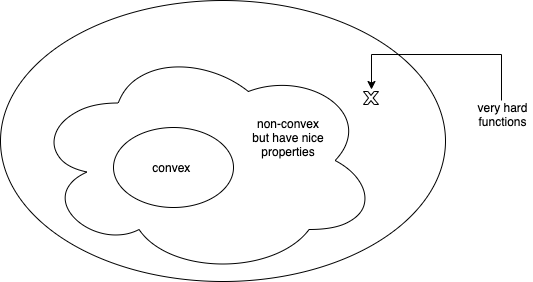
\includegraphics[scale = 0.5]{figures/landscape.png}
    \caption{Classification of different functions for optimization. The functions we optimize in deep learning seem to fall mostly within the middle cloud.}
    \label{lec10:fig:optimization}
\end{figure}

\begin{figure}[ht!]
    \centering
    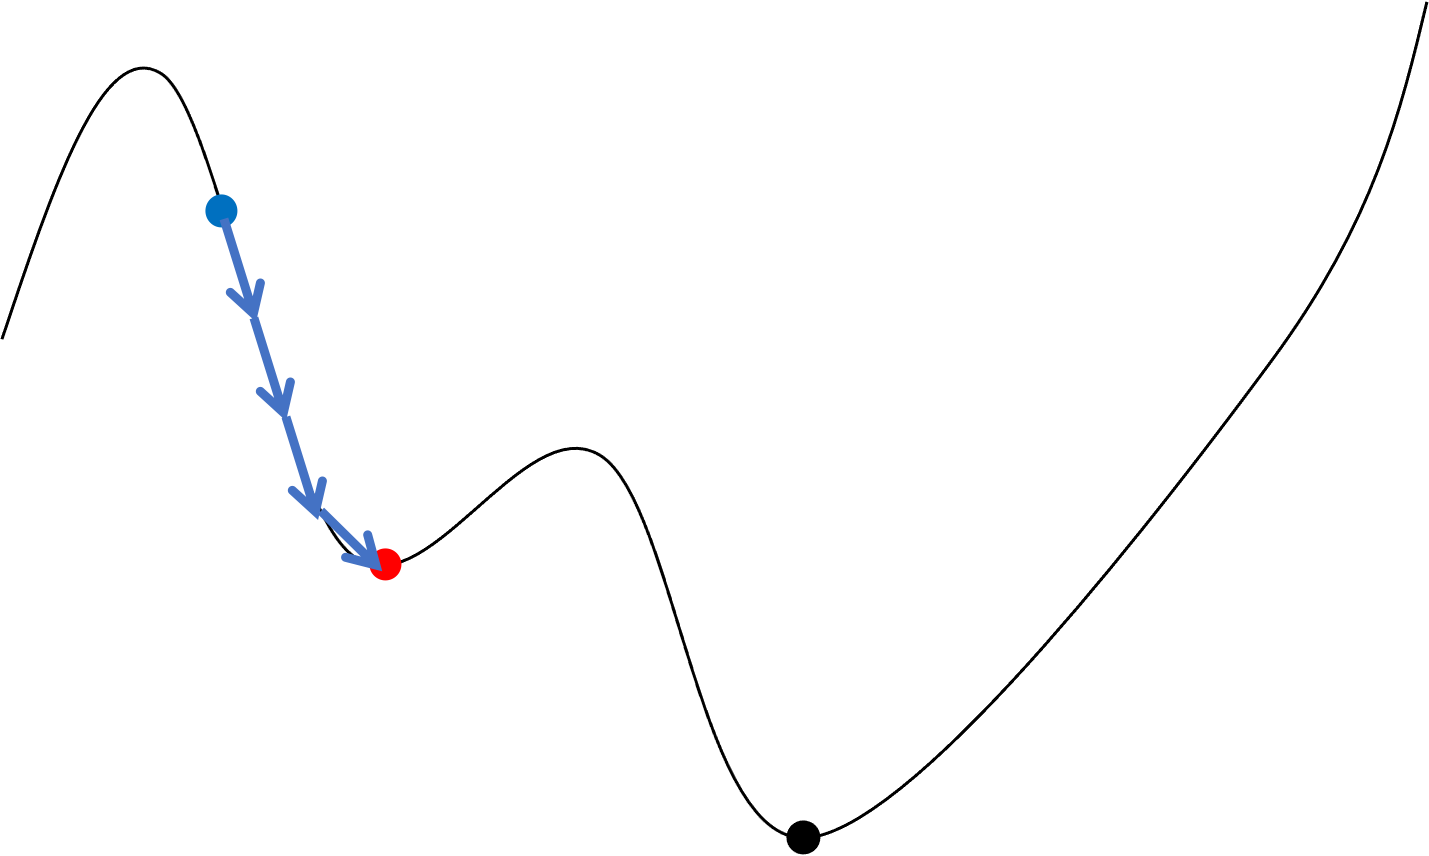
\includegraphics[scale = 0.3]{figures/gradient_descent.png}
    \caption{Illustration of how gradient descent does not always find the global minimum. In the picture, gradient descent initialized at the blue point only makes it to the local minimum at the red point: it does not find the global minimum at the black point.}
    \label{lec10:fig:gradient_descent}
\end{figure}
Before diving into details, we first highlight some observations that will be important to keep in mind when discussing optimization in deep learning. Suppose $g(\theta)$ is the loss function. Recall that the \textit{gradient descent (GD)} algorithm would do the following:
\begin{enumerate}
    \item $\theta_0$ := initialization
    \item $\theta_{t + 1} = \theta_t - \eta\nabla g(\theta_t)$, where $\eta$ is the step size.
\end{enumerate}
Here are some observations to :
\begin{enumerate}
    \item[] \textit{Observation 1}: Gradient descent can find a global minimum for convex functions\footnote{A more precise version of this claim is that gradient descent can find a point that has function value arbitrary close to the global minimal value. } but cannot always find the global minimum for any general continuous functions (see Figure \ref{lec10:fig:gradient_descent} for an illustration).
    \item[] \textit{Observation 2}: Finding the global minimum of general non-convex functions is NP-hard.
%    \item[] \textit{Observation 3}: Gradient descent .
    \item[] \textit{Observation 3}: The objective function in deep learning is non-convex., but empirically gradient descent/stochastic gradient descent typically finds an approximate global minimum of loss function in deep learning.
\end{enumerate}

These observations motivate the following two-step plan:

\begin{enumerate}
    \item Identify a large set of functions that stochastic gradient descent/gradient descent can solve.
    \item Prove that some of the loss functions in machine learning problems belong to this set. (Most of the effort will be spent here.)
\end{enumerate}
\textbf{Basic idea:} Gradient descent can find local minimum $+$ all local minima of $f$ are also global $\Rightarrow$ Gradient descent can find global minima.

\sec{Efficient convergence to (approximate) local minima} \label{sec:optim_convergence}
Let $f$ be a twice-differentiable function. We start with the following definition:
\begin{definition} [Local minimum of a function]
We say that $x$ is a \textit{local minimum} of a function $f$ if there exists an open neighborhood $N$ around $x$ such that in $N$, the function values are at least $f(x)$.
\end{definition}

Note that if $x$ is a local minimum of $f$, then $\nabla f(x) = 0$ and $\nabla^2 f(x) \succeq 0$. However, as the next example shows, the reverse is not true. When $\nabla f(x) = 0$ and $\nabla^2 f(x)$ vanishes in some direction (i.e. merely positive semi-definite instead of being strictly positive definite), higher-order derivatives start to matter.

\begin{example}
\label{lec10:ex:counterexample}
Consider the function $f(x_1, x_2) = x_1^2 + x_2^3$. $(x_1, x_2) = (0, 0)$ satisfies $\nabla f(x) = 0$ and $\nabla^2 f(x)|_{(x_1, x_2) = (0, 0)} = \begin{bmatrix} 2 & 0 \\
0 & 0\end{bmatrix} \succeq 0$. However, if we move in the negative direction of $x_2$, we can decrease the function value. Hence, this example shows why $\nabla f(x) = 0$ and $\nabla^2 f(x) \succeq 0$ does not imply that $x$ is a local minimum.
\end{example}

It is generally not easy to verify if a point is a local minimum. In fact, we have the following theorem regarding the computational tractability:
\begin{theorem}
\label{lec10:thm:np_hard}
It is NP-hard to check whether a point is a local minimum or not \cite{murty1987}. In addition, Hillar and Lim \cite{hillar2013} show that a degree four polynomial is NP-hard to optimize.
\end{theorem}

\subsec{Strict-saddle condition}
Theorem~\ref{lec10:thm:np_hard} forces us to consider more specific types of functions to be able to obtain computational tractability. To this end, we define the following \textit{strict-saddle condition}:

\begin{definition} [Strict-saddle condition \cite{lee2016}]
For positive $\alpha, \beta, \gamma$, we say that $f: \R^d \mapsto \R$ is \textit{$(\alpha, \beta, \gamma)$-strict-saddle} if every $x \in \bbR^d$ satisfies one of the following:
\begin{enumerate}
    \item $\|\nabla f(x)\|_2 \geq \alpha$.
    \item $\lambda_{\min}(\nabla^2 f(x)) \leq -\beta$.
    \item $x$ is $\gamma$-close to a local minimum $x^*$ in Euclidean distance, i.e. $\|x - x^*\|_2 \leq \gamma$.
\end{enumerate}
\end{definition}

Intuitively speaking, this definition is saying if a point has zero gradient and positive semi-definite Hessian, it must be close to a local minimum, i.e. there is no pathological case like Example \ref{lec10:ex:counterexample}.

We have the following theorem for functions that satisfy strict-saddle condition:

\begin{theorem} [Informally stated]
If $f$ is $(\alpha, \beta, \gamma)$-strict-saddle for some positive $\alpha, \beta, \gamma$, then many optimizers (e.g. gradient descent, stochastic gradient descent, cubic regularization) can converge to a local minimum with $\epsilon$-error in Euclidean distance in time $poly \left(d, \frac{1}{\alpha}, \frac{1}{\beta}, \frac{1}{\gamma}, \frac{1}{\epsilon}\right)$.
\end{theorem}

Therefore, if all local minima are global minima and the function satisfies the strict-saddle condition, then optimizers can converge to a global minimum with $\epsilon$-error in polynomial time. (See Figure \ref{lec10:fig:strict-saddle} for an example of a function whose local minima are all global minima.) The next theorem expresses this concretely by being explicit about the strict-saddle condition:

\begin{theorem}
Suppose $f$ is a function that satisfies the following condition: $\exists  \ \epsilon_0, \tau_0, c > 0$ such that if $x \in \bbR^d$ satisfies $\|\nabla f(x)\|_2 \leq \epsilon < \epsilon_0$ and $\nabla^2 f(x) \succeq -\tau_0I$, then $x$ is $\epsilon^c$-close to a global minimum of $f$. Then many optimizers can converge to a global minimum of $f$ up to $\delta$-error in Euclidean distance in time $poly\left(\frac{1}{\delta}, \frac{1}{\tau_0}, d \right)$.
\end{theorem}

\begin{figure}[ht!]
    \centering
    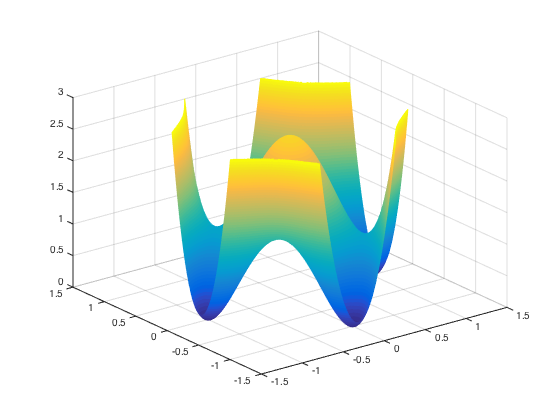
\includegraphics[scale = 0.5]{figures/localmin.png}
    \caption{A two-dimensional function with the property that all local minima are global minima. It also satisfies the strict-saddle condition because all the saddle points have a strictly negative curvature in some direction.}
    \label{lec10:fig:strict-saddle}
\end{figure}

\sec{All local minima are global minima: two examples} \label{sec:two_optim_examples}
So far, we have focused on general results. Next, we give two concrete examples that have the property that all local minima are global minima: (i) principal components analysis (PCA)/matrix factorization/linearized neural nets, and (ii) matrix completion. \tnote{need some quick literature survey; Tengyu will add}%There is a rich literature on this topic and 

\subsec{Principal components analysis (PCA)}
Let matrix $M \in \bbR^{d \times d}$ be symmetric and positive semi-definite. Consider the problem of finding the best rank-1 approximation of the matrix $M$. The objective function here is non-convex:
\begin{equation}
    \min_{x \in \bbR^d}g(x) \triangleq \frac{1}{2}\|M - xx^\top \|_F^2.
\end{equation}

\begin{theorem}
All local minima of $g$ are global minima (even though $g$ is non-convex).
\end{theorem}

\begin{remark}
For $d = 1$, $g(x) = \frac{1}{2}(m - x^2)^2$ for some constant $m$. Figure~\ref{lec10:fig:pca_objective} below shows such an example. We can see that all local minima are indeed global minima.
\end{remark}

\begin{figure}[ht!]
    \centering
    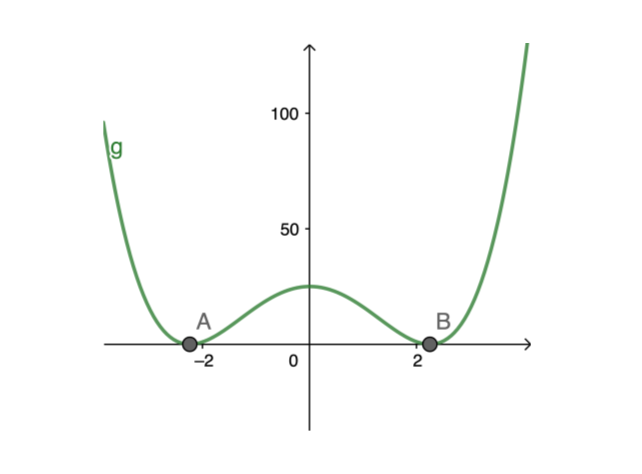
\includegraphics[scale = 0.4]{figures/pca.png}
    \caption{Objective function for principal components analysis (PCA) when $d = 1$.}
    \label{lec10:fig:pca_objective}
\end{figure}

\begin{proof}

\textit{Step 1: Show that all stationary points must be eigenvectors.} From HW0, we know that $\nabla g(x) = -(M - xx^\top )x$, hence
\begin{equation}\label{lec10:eqn:pca-firstorder}
\nabla g(x) = 0 \implies Mx = \|x\|_2^2\cdot x,
\end{equation}
which implies that $x$ is an eigenvector of $M$ with eigenvalue $\|x\|_2^2$. From the Eckart–Young–Mirsky theorem we know the global minimum (i.e. the best rank-1 approximation) is the eigenvector with the largest eigenvalue.

\textit{Step 2: Show that all local minima must be eigenvectors of the largest eigenvalue.} We use the second order condition for this. For $x$ to be a local minimum we need $\nabla^2g(x) \succeq 0$, which means for any $v \in  \bbR^d$, 
\begin{equation}
\langle v, \nabla^2g(x) v \rangle \geq 0.
\end{equation}
To compute $\langle v, \nabla^2g(x) v \rangle$, we use the following trick: expand $g(x + v)$ into $g(x) + \text{linear term in } v + \text{quadratic term in } v$, then the quadratic term will be $\frac{1}{2}\langle v, \nabla^2g(x) v \rangle$ (see HW0 Problem 2d for an example). Using this trick, we get 

\begin{align}
    g(x+v) &= \frac{1}{2}\|M - (x+v)(x+v)^\top \|_F^2 \\
           &= \frac{1}{2}\|M-xx^\top\|_F^2 - \langle M-xx^\top , xv^\top + vx^\top\rangle + \frac{1}{2}\langle xv^\top + vx^\top , xv^\top + vx^\top \rangle \nonumber \\
          & \quad -\langle M-xx^\top, vv^\top\rangle + \text{higher order terms in }v.
\end{align}
Hence, we have 
\begin{align}
    \frac{1}{2}\langle v, \nabla^2g(x) v \rangle & = \frac{1}{2}\langle xv^\top + vx^\top, xv^\top + vx^\top \rangle
          -\langle M-xx^\top, vv^\top\rangle  \\
          &= \langle x, v\rangle^2 + \|x\|_2^2\|v\|_2^2 - v^ Mv + \langle x, v\rangle^2 \\
          & = 2\langle x, v\rangle^2 + \|x\|_2^2\|v\|_2^2 - v^\top Mv.
\end{align}

Picking $v = v_1$, the unit eigenvector with the largest eigenvalue (denoted $\lambda_1$), for $x$ to be a local minimum it must satisfy 
\begin{equation}
\langle v_1, \nabla^2g(x) v_1 \rangle = 2\langle x, v_1 \rangle^2 - v_1^\top Mv_1 + \|x\|_2^2 \geq 0.
\end{equation}

Note that by \eqref{lec10:eqn:pca-firstorder}, all our candidates for local minima are eigenvectors of $M$ so naturally we have two cases:
\begin{itemize}
\item \textit{Case 1: $x$ has eigenvalue $\lambda_1$}. Then x is the global minimum (by the Eckart–Young–Mirsky theorem).
\item \textit{Case 2: $x$ has eigenvalue $\lambda < \lambda_1$}. Then we know $x$ and $v_1$ are orthogonal (eigenvectors with different eigenvalues are always orthogonal), hence 
\begin{equation}
2\langle x, v_1 \rangle^2 - v_1^\top Mv_1 + \|x\|_2^2 = 0  -\lambda_1 + \lambda \geq 0,
\end{equation}
which implies $\lambda \geq \lambda_1$, a contradiction. 
\end{itemize}

In summary, if $x$ is a stationary point and $x$ is not a global minimum, then moving in the direction of $v_1$ would lead to second-order improvement and $x$ cannot be a local minimum. 
\end{proof}
